\chapter{Release 2: Automatisation des tests fonctionnels et SEO, génération des rapports et déploiement}
\renewcommand{\thesection}{\arabic{section}}
\begin{justify}
    \vspace{-0.8cm}
    \section*{\texorpdfstring{Introduction}{Introduction}}
    \addcontentsline{toc}{chapter}{\textbf{Introduction}}
    Dans le chapitre précédent, nous avons décrit le premier sprint et abouti à une première version de l’application. Dans ce chapitre, nous commencerons à travailler sur le deuxième incrément, qui sera principalement axé sur l'automatisation des tests fonctionnels, la gestion des résultats, la génération de rapports, la création de tableaux de bord et la gestion des utilisateurs.
    \section{Planification de la release 2}
    Cette seconde itération a permis d'intégrer les fonctionnalités avancées et d'assurer la finalisation du projet. La release 2 s'est déroulée selon l'organisation suivante:
\begin{itemize}[label=$\bullet$]
    \item \textbf{Sprint 2.1 — Intégration des fonctionnalités clés de gestion des scans (25 jours ouvrés)} : du 16 avril 2025 au 21 mai 2025.
    \item \textbf{Sprint 2.2 — Finalisation et déploiement de l’application (22 jours ouvrés)}: du 22 mai 2025 au 23 juin 2025.
\end{itemize}
    \section{Sprint 2.1 : Intégration des fonctionnalités clés de gestion des scans}
Ce sprint s’est concentré sur l’implémentation des fonctionnalités principales liées à la gestion des différents types de scans :
\begin{itemize}[label=$-$]
    \item \textbf{Gestion des scans fonctionnels} : développement des modules permettant de lancer et gérer les tests fonctionnels sur les sites web.
    \item \textbf{Gestion des analyses SEO} : mise en place des outils d’analyse SEO pour évaluer la performance des sites.
\end{itemize}
Ce sprint a permis d’enrichir l’application avec des fonctions essentielles pour l’analyse complète des sites web.

\subsection{Backlog du sprint 2.1}  
Dans cette section, nous présenterons le Backlog du sprint 2, illustré dans le tableau \ref{tab:backlogS2}, en tenant compte des modifications et ajustements apportés depuis le sprint précédent.
\begin{landscape}
    \renewcommand{\arraystretch}{1}
    \begin{spacing}{0.98}
        \begin{longtable}{|p{0.5cm}|p{3cm}|p{6cm}|p{0.9cm}|p{7.8cm}|p{0.6cm}|p{0.6cm}|p{1.2cm}|}
            \caption{Backlog du sprint 2.1} \label{tab:backlogS2} \\\hline
            \rowcolor{gray!20}
            \textbf{\small ID US} & 
            \multicolumn{1}{c|}{\textbf{\small User Story}} & 
            \multicolumn{1}{c|}{\textbf{\small Description}} & 
            \textbf{\small ID tâche}& 
            \multicolumn{1}{c|}{\textbf{\small Tâches}} & 
            \multicolumn{1}{c|}{\textbf{\small Priorité}} & 
            \multicolumn{1}{c|}{\textbf{\small Risques}} & 
            \textbf{\small Estim-ation(j)} \\\hline          
            % ----------- SCANS Fonctionnels -----------------
            \hline  
            \rowcolor{blue!20}
			\multicolumn{8}{|c|}{\textbf{EPIC 5: Gestion des tests fonctionnels d'un site web}} \\\hline
                5.1 & Gérer les scénarios de test "Workflow".
                    & En tant que testeur, je dois gérer les scénarios de test pour assurer la couverture fonctionnelle. 
                    & 5.1.A \newline\vspace{0.5cm} 5.1.B
                    &
                    - Ajouter la possibilité de créer, modifier, exécuter et supprimer des scénarios de test. \newline
                    - Afficher les résultats des scénarios.
                    & Élevée & Moyenne & 2 \\ \hline            
                 5.2 & Gérer les cas de test associés à chaque scénario de test. 
                    & En tant que testeur, je dois manipuler les cas de test pour valider les différentes fonctionnalités. 
                    & 5.2.A \newline\vspace{0.5cm} 5.2.B 
                    &
                    - Implémenter la création, la modification, la suppression et l'exécution de cas de test pour chaque scénario. \newline
                    - Afficher les résultats et les erreurs liées aux cas de test.
                    & Élevée & Moyenne & 2 \\ \hline
                
                5.3 & Gérer les étapes associées à chaque cas de test. 
                    & En tant que testeur, je dois gérer les étapes de test pour garantir le bon déroulement des tests. 
                    & 5.3.A \newline\vspace{0.5cm} 5.3.B
                    &
                    - Implémenter la gestion des étapes de test pour chaque cas. \newline
                    - Ajouter un suivi de l'état des étapes de test exécutées.
                    & Moyenne & Basse & 2 \\ \hline
                
                5.4 & Lancer un scan de test fonctionnel. 
                    & En tant que testeur, je souhaite exécuter automatiquement des tests fonctionnels afin de vérifier la fiabilité de l'application.
                    & 5.4.A \newline\vspace{0.5cm} 5.4.B
                    &
                    - Ajouter la fonctionnalité pour démarrer un scan de test fonctionnel. \newline
                    - Générer et afficher les rapports de tests après exécution.
                    & Moyenne & Basse & 2 \\ \hline
                \hline
                5.5 & Planifier l'exécution les scans fonctionnels
                    & En tant que testeur, je souhaite planifier l'automatisation des tests fonctionnels pour garantir une exécution régulière.
                    & 5.5.A \newline\vspace{0.5cm} 5.5.B 
                    & - Ajouter un système de planification (scheduler). \newline
                      - Permettre l'exécution automatique selon un planning défini.
                    & Élevée & Moyenne & 2 \\\hline
                
                5.6 & Suivre l'exécution fonctionnels en temps réel
                    & En tant que testeur, je veux suivre les tests via WebSocket pour visualiser la progression.
                    & 5.6.A 
                    & - Intégration WebSocket pour monitoring en temps réel.
                    & Moyenne & Basse & 1 \\\hline
                
                5.7 & Visualiser les résultats des tests fonctionnels
                    & En tant que testeur, je souhaite consulter les résultats des tests exécutés pour corriger les bugs.
                    & 5.7.A \newline\vspace{0.5cm} 5.7.B 
                    & - Créer une interface pour visualiser les anomalies et logs de tests. \newline
                      - Ajouter des filtres et détails pour chaque scénario ou cas de test.
                    & Élevée & Moyenne & 2 \\\hline
                
                5.8 & Intégrer les résultats de tests avec Jira, Slack et email
                    & En tant que testeur, je souhaite envoyer les anomalies détectées vers Jira, Slack et email automatiquement.
                    & 5.8.A \newline\vspace{0.5cm} 5.8.B \newline 5.8.C
                    & - Ajouter une intégration API avec Jira pour la création de tickets.\newline
                    - Envoi automatisé des résultats via Slack. \newline
                    - Envoi des rapports par email.
                    & Moyenne & Moyenne & 2 \\\hline
                5.9 & Gérer l'historique et télécharger les rapports.
                    & En tant que testeur, je souhaite consulter l'historique des rapports des scans fonctionnels et les exporter.
                    & 5.9.A \newline\vspace{0.5cm} 5.9.B
                    & - Stocker l'historique des rapports (base de données ou fichiers). \newline
                      - Exporter les rapports HTML, JSON, CSV, PDF, ZIP.
                    & Élevée & Moyenne & 2 \\\hline
         % ----------- EPIC 6: SEO -----------------
                \hline
                \rowcolor{blue!20}
                \multicolumn{8}{|c|}{\textbf{EPIC 6: Gestion des analyses SEO d'un site web}} \\\hline
                
                6.1 & Lancer une analyse SEO complète
                    & En tant que testeur, je veux analyser le site cible pour évaluer sa qualité SEO.
                    & 6.1.A \newline\vspace{0.5cm} 6.1.B 
                    & - Implémenter l'analyse SEO : balises, performances, mots clés... \newline
                      - Calculer un score global SEO.
                    & Élevée & Moyenne & 2 \\\hline
                
                6.2 & Identifier les technologies et mots-clés
                    & En tant qu'auditeur, je veux connaître les frameworks utilisés et les mots-clés extraits.
                    & 6.2.A 
                    & - Extraire les CMS, JS, langages backend et mots-clés textuels.
                    & Moyenne & Moyenne & 1 \\\hline
                
                6.3 & Générer une capture d'écran de la page cible
                    & En tant que testeur, je veux voir un aperçu visuel de la page analysée.
                    & 6.3.A 
                    & - Générer automatiquement une capture d'écran avec Puppeteer ou outil équivalent.
                    & Moyenne & Faible & 1 \\\hline
                
                6.4 & Suivre l'analyse SEO en temps réel
                    & En tant que testeur, je souhaite voir la progression du scan SEO en live.
                    & 6.5.A 
                    & - Intégration WebSocket pour progression de l'analyse.
                    & Basse & Faible & 1 \\\hline
                
                6.5 & Visualiser et exploiter les résultats SEO
                    & En tant que testeur, je veux lire les points forts et axes d'amélioration SEO.
                    & 6.5.A 
                    & - Créer une interface de visualisation du rapport SEO et classer par catégorie : technique, contenu, performance...
                    & Élevée & Moyenne & 2 \\\hline
                
                6.6 & Intégration Jira / Slack / Email pour SEO
                    & En tant qu'auditeur, je veux notifier et suivre les anomalies SEO détectées.
                    & 6.6.A \newline\vspace{0.5cm} 6.6.B \newline 6.6.C
                    & - Créer des tickets Jira automatiquement pour problèmes critiques. \newline
                      - Notification via Slack. \newline
                      - Envoi du rapport SEO par email.
                    & Moyenne & Faible & 2 \\\hline
                6.7 & Historique et export des rapports SEO
                    & En tant que testeur, je veux pouvoir retrouver et télécharger les rapports SEO précédents.
                    & 6.7.A 
                    & - Gérer l'historique et exporter les rapports (HTML, JSON, PDF, ZIP, CSV).
                    & Moyenne & Moyenne & 1 \\\hline          
            \rowcolor{gray!20}
			\multicolumn{7}{|c|}{TOTAL} &  25 \\
            \hline 
        \end{longtable}
    \end{spacing}
\end{landscape}

\subsection{Analyse du sprint 2.1}
Dans cette phase nous allons présenter le diagramme de cas d’utilisation de ce sprint. Ensuite, nous mettons en disposition les descriptions textuelles de certains cas d’utilisation.
\subsubsection{ Diagramme de cas d’utilisation du sprint 2.1}
    La figure \ref{fig:caseS21} illustre le diagramme de cas d’utilisation pour le sprint 2.1.
        \begin{figure}[H]
            \centering
            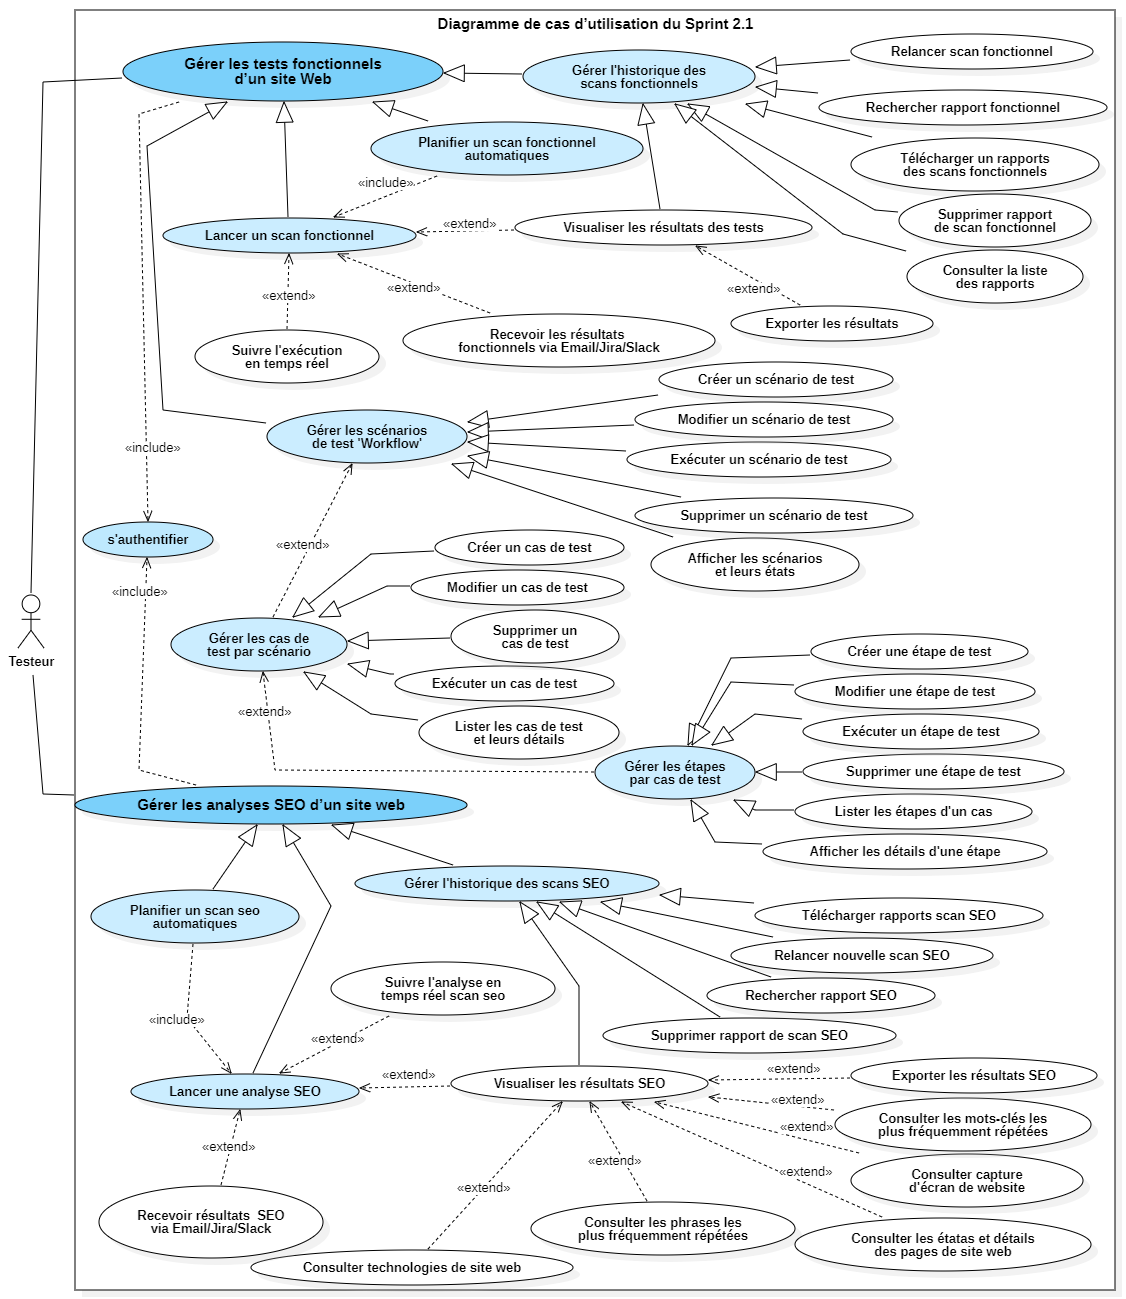
\includegraphics[width=\linewidth]{chapitres/ch4Sp2/section/sprint2.1/img/LastUseCaseSprint2.1.png}
            \caption{Diagramme de cas d'utilisations du sprint 2.1}
            \label{fig:caseS21}
        \end{figure}
\subsection{Raffinement des cas d'utilisation}
    \subsubsection{Description textuelle du cas d'utilisation « Lancer un scan fonctionnel »}
        Le tableau ~\ref{tab:descScanFonctionnel} présente la description textuelle du cas d'utilisation "Lancer un scan fonctionnel".
                \begin{spacing}{1}
                    \begin{longtable}{|p{0.12\linewidth}|p{0.85\linewidth}|}
                        \caption{Description textuelle du cas d'utilisation : Lancer un scan fonctionnel}
                        \label{tab:descScanFonctionnel}\\
                        \hline
                        \textbf{Titre} & Lancer un scan fonctionnel \\
                        \hline
                        \textbf{Acteur} & Testeur \\
                        \hline
                        \textbf{Résumé} & Ce cas d'utilisation permet au testeur de déclencher l'exécution automatisée d'un ensemble de scénarios de test fonctionnels sur une application web afin de valider le comportement de l'application avec un suivi en temps réel. \\
                        \hline
                        \textbf{Pré-conditions} & 
                        \begin{minipage}{0.83\textwidth}
                             \vspace{0.05cm}
                            \begin{itemize}[left=0cm]
                                \item[\textbullet] L'utilisateur est authentifié en tant que Testeur
                                \item[\textbullet] Au moins un scénario de test existe dans le système
                            \end{itemize}
                        \end{minipage} \\
                        \hline
                        \textbf{Post-conditions} & 
                        \begin{minipage}{0.83\textwidth}
                            \vspace{0.1cm}
                            \textbf{En cas de succès :}
                            \begin{itemize}[left=0cm]
                                \item[\textbullet] Le scan fonctionnel est lancé avec succès avec un identifiant unique de scan est généré
                                \item[\textbullet] Les notifications sont envoyées selon la configuration
                                \item[\textbullet] L'historique est mis à jour
                            \end{itemize}
                            \textbf{En cas d'échec :}
                            \begin{itemize}[left=0cm]
                                \item[\textbullet] Le scan n'est pas lancé et un message d'erreur explicite est affiché
                                \item[\textbullet] Aucune notification n'est envoyée
                            \end{itemize}
                            \vspace{0.1cm}
                        \end{minipage} \\
                        \hline
                        \textbf{Scénario nominal} & 
                        \begin{minipage}{0.83\textwidth}
                            \vspace{0.1cm}
                            \begin{enumerate}[label=\arabic*.]
                                \item Le testeur accède à l'interface de lancement de scan
                                \item Le système affiche les scénarios disponibles
                                \item Le testeur sélectionne les scénarios à exécuter.
                                \item Le testeur confirme le lancement
                                \item Le système génère un ID unique, crée une session d'exécution et met à jour le statut à "En cours"
                                \item Le système envoie les notifications de début
                                \item Le système lance l'exécution des tests en arrière-plan
                                \item Le système active le suivi en temps réel
                                \item Si l'envoi des rapports est configuré, le système crée automatiquement des tickets Jira ou envoie un message via Slack ou par email, selon le type de configuration.
                            \end{enumerate}
                            \vspace{0.1cm}
                        \end{minipage}\\
                        \hline
                        \textbf{Scénario d'erreur} &
                        \begin{minipage}{0.83\textwidth}
                            \vspace{0.1cm}
                            \begin{itemize}[left=0cm]
                                \item[\textbullet] \textbf{Étape 3 (Aucun scénario sélectionné):}
                                \begin{itemize}[label=\ding{56}]
                                    \item Le système affiche un message d'erreur
                                    \item Le système invite le testeur à sélectionner au moins un scénario
                                    \item Retour à l'étape 3
                                \end{itemize}
                            \end{itemize}
                            \vspace{0.1cm}
                        \end{minipage}\\
                        \hline
                    \end{longtable}
                \end{spacing}   
    \vspace{-0.2cm}
    \subsubsection{Description textuelle du cas d’utilisation «Lancer une analyse SEO»}    
            Le tableau ~\ref{tab:descAnalyseSEO} présente la description textuelle du cas d’utilisation "Lancer une analyse SEO".
            \begin{spacing}{1.2}
                \begin{longtable}{|p{0.12\linewidth}|p{0.85\linewidth}|}
                \caption{Description textuelle du cas d’utilisation : Lancer une analyse SEO}
                \label{tab:descAnalyseSEO}\\
                \hline
                \textbf{Titre} & Lancer une analyse SEO\\ 
                \hline
                \textbf{Acteur} & Testeur \\
                \hline
                \textbf{Résumé} & Ce cas d'utilisation permet au testeur de lancer une analyse d'un site web afin d'évaluer sa qualité SEO à travers différents indicateurs techniques et de contenu. \\
                \hline
                \textbf{Pré-conditions} &
                Le testeur doit avoir accès à l’interface de scan, et l’URL du site cible doit être valide et accessible publiquement. \\
                \hline
                \textbf{Post-conditions} &
                Un rapport SEO est généré, incluant les résultats de l’analyse (balises, mots clés, performances…) et un score global est calculé. \\
                \hline
                \textbf{Scénario nominal} &
                \begin{minipage}{0.83\textwidth}
                \vspace{0.1cm}
                \begin{enumerate}[label=\arabic*.]
                \item Le testeur accède à l’interface d’analyse SEO.
                \item Il saisit ou colle l’URL du site à analyser.
                \item Il lance l’analyse en cliquant sur le bouton dédié.
                \item Le système récupère les données du site (HTML, métadonnées, performances…).
                \item Le système effectue les vérifications SEO : balises manquantes, densité des mots clés, temps de chargement, structure, etc.
                \item Le système calcule un score global basé sur les critères définis.
                \item Un rapport d’analyse détaillé est généré et affiché à l’écran.
                \end{enumerate}
                \vspace{0.1cm}
                \end{minipage}\\
                \hline
                \textbf{Scénario d’erreur} &
                \begin{minipage}{0.83\textwidth}
                \vspace{0.1cm}
                \begin{itemize}[left=0cm]
                \item[\textbullet] \textbf{Étape 2 (URL invalide):}
                \begin{itemize}[label=\ding{56}]
                \item Le système affiche un message d’erreur indiquant que l’URL saisie est invalide.
                \end{itemize}
                    \item[\textbullet] \textbf{Étape 4 (Échec de récupération de données):}
                    \begin{itemize}[label=\ding{56}]
                        \item Le système affiche une alerte mentionnant l’échec de connexion au site ou un temps d’attente dépassé.
                    \end{itemize}
                
                    \item[\textbullet] \textbf{Étape 5 (Erreur d’analyse):}
                    \begin{itemize}[label=\ding{56}]
                        \item Si une erreur technique survient lors du parsing SEO, une notification avec détail de l’erreur est proposée au testeur.
                    \end{itemize}                  
                \end{itemize}
                \vspace{0.1cm}
                \end{minipage}\\
                \hline
                \end{longtable}
            \end{spacing}            
        \vspace{-0.3cm}

\subsection{Conception du sprint 2.1}
Dans cette section, nous présentons la conception détaillée des fonctionnalités développées au cours du sprint, à travers des diagrammes de classes et de séquences.
\subsubsection{Diagramme de classe du Sprint 2.1}
    Ce diagramme vient enrichir l'architecture définie au sprint précédent, en intégrant la gestion des tests fonctionnels automatisés et les analyses SEO avancées.
    \begin{figure}[H]
        \centering
        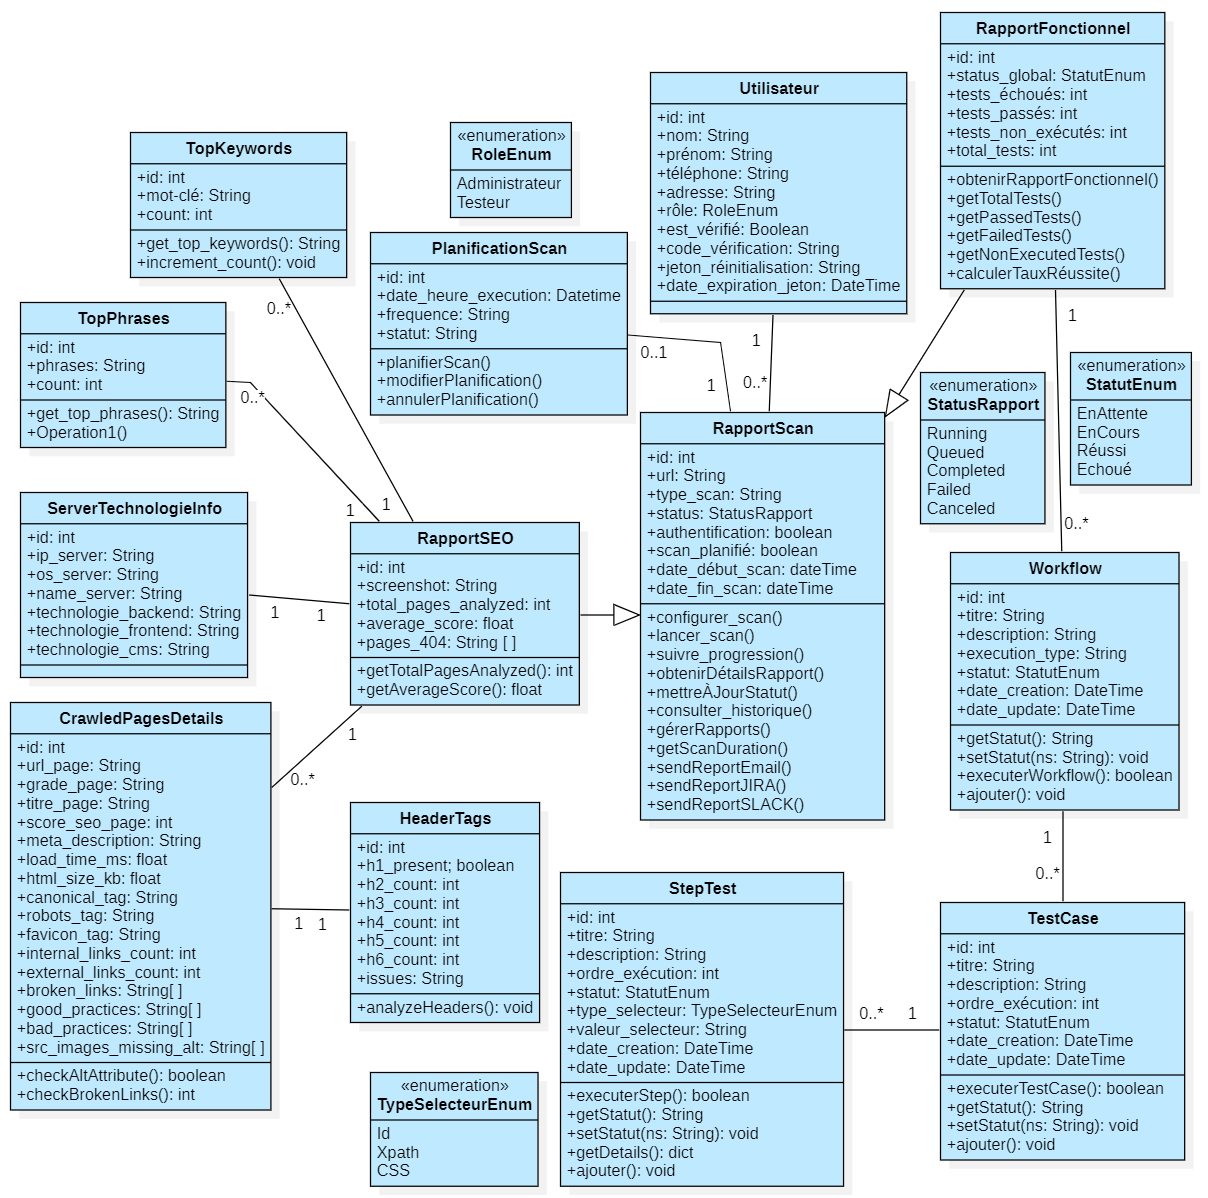
\includegraphics[width=\linewidth]{chapitres/ch4Sp2/section/sprint2.1/img/classeL2-SP2.1.png}
        \caption{Diagramme de classe du sprint 2.1}
        \label{fig:classsp2}
    \end{figure}
    \vspace{-0.7cm}
    Les principales classes modélisées du sprint 2.1 sont les suivantes:
    \begin{itemize}[label=$*$]
        \item \textbf{Utilisateur:} Classe représentant les utilisateurs du système.  
        \item \textbf{PlanficationScan:} Gère la planification des scans avec des fonctionnalités de programmation, modification et annulation des analyses automatisées.
        
        \item \textbf{RapportScan:} Classe principale pour les rapports de scan incluant la configuration, le lancement, le suivi de progression et la gestion des résultats d'analyse.
        
        \item \textbf{RapportSEO:} Spécialise les rapports pour l'analyse SEO avec des métriques spécifiques comme le nombre total de pages analysées et le score moyen.
        
        \item \textbf{RapportFonctionnel:} Représente les résultats des tests fonctionnels réalisés avec des informations sur le statut global, les différents tests effectués, et leur réussite ou échec.
        
        \item \textbf{TopKeywords:} Contient les mots-clés les plus importants extraits lors des analyses SEO, utilisés pour le suivi des performances et des tendances.
        
        \item \textbf{TopPhrases:} Contient les phrases clés les plus pertinentes issues de l'analyse SEO, servant à enrichir les rapports et améliorer le référencement.
        
        \item \textbf{ServerTechnologieInfo:} Fournit des détails sur les technologies serveur détectées, telles que les systèmes d'exploitation, CMS, frameworks front-end et back-end utilisés.
        
        \item \textbf{CrawledPagesDetails:} Représente les informations détaillées des pages web crawlées durant les scans(URL, score SEO associé, métriques de performance...).
        
        \item \textbf{HeaderTags:} Regroupe les métadonnées extraites des pages web, comme les balises Hn, les descriptions meta, et d'autres éléments influençant le référencement naturel.

        \item \textbf{Workflow:} Modélise la chaîne ou séquence d'exécution des tests automatisés, incluant la gestion du statut et des étapes du processus.
        
        \item \textbf{TestCase:} Définit un cas de test fonctionnel détaillé, incluant la description, l'ordre d'exécution, et les critères de réussite ou d'échec.
        
        \item \textbf{StepTest:} Représente une étape précise dans un scénario de test fonctionnel, avec un suivi du statut et des résultats partiels.
                
        \item \textbf{StatutEnum (énumération):} Définit les différents états possibles d'un test ou rapport (EnAttente, EnCours, Réussi, Échoué).
        
        \item \textbf{StatusRapport (énumération):} Spécifie les états des rapports de scan (Running, Queued, Completed, Failed, Canceled).
        
        \item \textbf{RoleEnum (énumération):} Définit les rôles des utilisateurs (Administrateur, Testeur).
        
        \item \textbf{TypeSelecteurEnum (énumération):} Définit les types de sélecteurs utilisés dans les tests (Id, Xpath, CSS).
    \end{itemize}
    Les associations entre classes dans Sprint 2.1 incluent:
    \begin{itemize}[label=$-$]
        \item Un \texttt{Utilisateur} peut avoir plusieurs \texttt{PlanficationScan} et \texttt{RapportScan} associés.
        \item Un \texttt{RapportFonctionnel} centralise plusieurs \texttt{Workflow}, chacun structurant l'exécution de plusieurs \texttt{TestCase}, eux-mêmes composés de plusieurs \texttt{StepTest}.
        \item Les \texttt{TopKeywords}, \texttt{TopPhrases}, \texttt{ServerTechnologieInfo} et \texttt{CrawledPagesDetails} sont liés à un \texttt{RapportSEO}.
        \item Les \texttt{HeaderTags} sont extraits pour chaque \texttt{CrawledPagesDetails}.
    \end{itemize}
    Cette modélisation structure le traitement et le suivi des tests fonctionnels et SEO, permettant une meilleure organisation et automatisation des analyses au sein du projet.



\subsubsection{Diagramme de séquence de conception du cas « Créer un scénario de test »}
Le diagramme présenté à la figure \ref{fig:add-workflow} illustre le déroulement du processus de création d’un nouveau scénario de test fonctionnel (\texttt{Workflow}). Ce processus est généralement initié par un utilisateur via l’interface de l’application et comprend la saisie des détails du scénario (nom, description). Une fois les informations saisies, le \texttt{Workflow} est créé et enregistré dans la base de données pour être exécuté ou modifié ultérieurement.

Une fois un \texttt{Workflow} créé, l'utilisateur est automatiquement redirigé vers une interface dédiée à la configuration du scénario. Cette page permet l’ajout des différents éléments constitutifs tels que les \texttt{TestCase} et les \texttt{StepTest}, tout en offrant des boutons de lancement pour exécuter directement le workflow ou ses tests associés. Cette interface assure ainsi une gestion fluide, interactive et complète du cycle de vie des scénarios de test.

\begin{figure}[H]
    \centering
    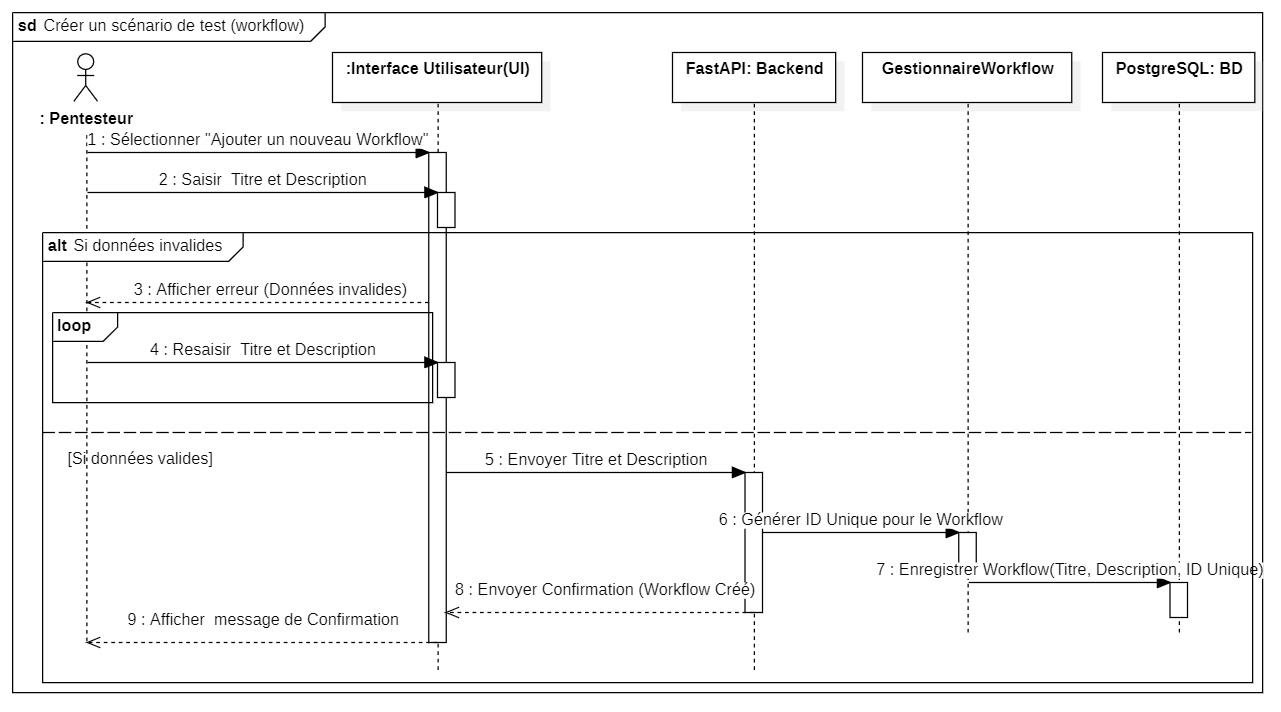
\includegraphics[width=\linewidth]{chapitres/ch4Sp2/section/sprint2.1/img/seq-workflow-creer.png}
    \caption{Diagramme de séquence de conception du cas « Créer un scénario de test »}
    \label{fig:add-workflow}
\end{figure}
\vspace{-0.4cm}

    

\subsection{Réalisation du sprint 2.1}
Dans cette section, nous présentons les principales interfaces développées durant ce sprint 2.1, en commençant par la gestion des tests fonctionnels, puis les interfaces liées à l'analyse SEO.
\begin{itemize}[label=$\bullet$]
    \item \textbf{Interface centralisée de gestion des tests fonctionnels:} La figure \ref{fig:interface-tests-fonctionnels}\footnote{Voir annexe E: Figure \ref{fig:interface-tests-fonctionnels}} illustre une interface unifiée dédiée à la gestion complète des tests fonctionnels. Elle permet à l’utilisateur de gérer l’ensemble du processus de test, depuis la création des scénarios jusqu’à l’exécution des tests. L’interface offre les fonctionnalités suivantes: création, modification, suppression et exécution des scénarios de test ; gestion des cas de test associés à chaque scénario, avec affichage des résultats et erreurs ; définition des étapes composant chaque cas de test, avec une visualisation détaillée des actions à réaliser et de leur statut ; enfin, lancement et suivi en temps réel des scans fonctionnels. Cette interface vise à centraliser et simplifier l’ensemble du cycle de vie des tests fonctionnels.
    \item \textbf{Interface de planification des scans fonctionnels}:
    La figure \ref{fig:planification-tests}\footnote{Voir annexe E: Figures \ref{fig:planification-tests}} illustre la fonctionnalité de planification de scans. Cette interface permet de configurer des exécutions automatiques selon une fréquence prédéfinie.
    
    \item \textbf{Interface de suivi en temps réel des exécutions fonctionnelles}:
    La figure \ref{fig:realtime-fonctionnel}\footnote{Voir annexe E: Figures \ref{fig:realtime-fonctionnel}} affiche une vue dynamique basée sur WebSocket pour suivre en direct l'exécution des tests.
    
    \item \textbf{Interface de visualisation des résultats fonctionnels}:
    La figure \ref{fig:resultats-fonctionnels}\footnote{Voir annexe E: Figures \ref{fig:resultats-fonctionnels}} présente les anomalies détectées, les logs détaillés, ainsi que des filtres permettant une analyse par scénario ou cas de test.
    
    \item \textbf{Interface d’intégration des résultats fonctionnels avec Jira, Slack et Email}:
    La figure \ref{fig:integration-resultats}\footnote{Voir annexe E: Figures \ref{fig:integration-resultats}} illustre l’écran de configuration des services tiers pour l’envoi automatique des rapports fonctionnels.
    
    \item \textbf{Interface d’historique des rapports fonctionnels}:
    La figure \ref{fig:historique-fonctionnel}\footnote{Voir annexe E: Figures \ref{fig:historique-fonctionnel}} montre l’interface de consultation des rapports précédents, avec options de tri, téléchargement en formats HTML, PDF, ZIP, etc.
    
    \item \textbf{Interface de lancement d’analyse SEO}:
    La figure \ref{fig:lancer-seo}\footnote{Voir annexe E: Figures \ref{fig:lancer-seo}} présente la page d'exécution d’un scan SEO complet, incluant balises, performance, accessibilité et mots-clés.
    
    \item \textbf{Interface d’identification des technologies et mots-clés SEO}:
    La figure \ref{fig:techno-keywords}\footnote{Voir annexe E: Figures \ref{fig:techno-keywords}} illustre les informations extraites sur les frameworks (CMS, JS, backend) et mots-clés présents sur la page cible.
    
    \item \textbf{Interface de capture d’écran SEO}:
    La figure \ref{fig:capture-seo}\footnote{Voir annexe E: Figures \ref{fig:capture-seo}} affiche l'aperçu visuel de la page scannée générée automatiquement à l’aide d’un outil de capture (ex: Puppeteer).
    
    \item \textbf{Interface de suivi temps réel du scan SEO}:
    La figure \ref{fig:seo-realtime}\footnote{Voir annexe E: Figures \ref{fig:seo-realtime}} montre l’évolution du scan SEO en temps réel grâce à WebSocket, avec visualisation de la progression.
    
    \item \textbf{Interface de visualisation des résultats SEO}:
    La figure \ref{fig:resultats-seo}\footnote{Voir annexe E: Figures \ref{fig:resultats-seo}} permet de consulter les résultats d’analyse SEO, classés par catégorie: contenu, technique, performance.
    
    \item \textbf{Interface d’intégration SEO avec Jira, Slack et Email}:
    La figure \ref{fig:integration-seo}\footnote{Voir annexe E: Figures \ref{fig:integration-seo}} permet la configuration des intégrations pour automatiser l’envoi des alertes SEO détectées.
    
    \item \textbf{Interface d’historique des rapports SEO}:
    La figure \ref{fig:historique-seo}\footnote{Voir annexe E: Figures \ref{fig:historique-seo}} fournit un tableau listant les rapports d’analyse SEO archivés, avec fonctionnalités d’export dans différents formats.
\end{itemize}




   % \item \textbf{Interface de la gestion des scénarios de test}:
    % La figure \ref{fig:scenario-test}\footnote{Voir annexe E: Figures \ref{fig:scenario-test}} illustre l’interface permettant de créer, modifier, exécuter ou supprimer des scénarios de test fonctionnels. L’utilisateur peut y consulter l’ensemble des scénarios définis, visualiser leurs statuts, et lancer leur exécution.
    
    % \item \textbf{Interface de gestion des cas de test}:
    % La figure \ref{fig:cas-test}\footnote{Voir annexe E: Figures \ref{fig:cas-test}} montre l’interface dédiée à la gestion des cas de test liés à chaque scénario. Elle permet d’ajouter, modifier ou supprimer des cas, tout en affichant les résultats et erreurs d’exécution.
    
    % \item \textbf{Interface de gestion des étapes de test}:
    % La figure \ref{fig:etapes-test}\footnote{Voir annexe E: Figures \ref{fig:etapes-test}} représente l’interface utilisée pour gérer les étapes constituant chaque cas de test. Elle fournit une vue détaillée des actions à exécuter ainsi que leur statut d'exécution.
    
    % \item \textbf{Interface de lancement des tests fonctionnels}:
    % La figure \ref{fig:lancer-scan-fonctionnel}\footnote{Voir annexe E: Figures \ref{fig:lancer-scan-fonctionnel}} montre la page qui permet de démarrer un scan fonctionnel. L'utilisateur peut choisir un scénario, lancer son exécution et suivre sa progression.
    

    \section{Sprint 2.2 : Finalisation et déploiement de l’application}
Ce sprint a permis de finaliser les fonctionnalités avancées et d’assurer la mise en production :
\begin{itemize}[label=$-$]
    \item \textbf{Gestion des scans multiples} : intégration des scans fonctionnels, sécurité et SEO dans une interface unifiée.
    \item \textbf{Visualisation des statistiques via le tableau de bord} : développement du tableau de bord pour un suivi clair des analyses.
    \item \textbf{Gestion des rapports des analyses effectuées} : mise en place des fonctionnalités de consultation et export des rapports.
    \item \textbf{Déploiement de l’application} : préparation et exécution du déploiement final en environnement de production.
\end{itemize}
Ce sprint a permis d’achever le projet en offrant une application complète et opérationnelle.

\subsection{Backlog du sprint 2.2}  
Dans cette section, nous présenterons le Backlog du sprint 2.2, illustré dans le tableau \ref{tab:backlogS22}, en tenant compte des modifications et ajustements apportés depuis le sprint précédent.
\begin{landscape}
    \renewcommand{\arraystretch}{1.1}
    \begin{spacing}{0.98}
        \begin{longtable}{|p{0.6cm}|p{3cm}|p{5.2cm}|p{1cm}|p{8.2cm}|p{0.6cm}|p{0.6cm}|p{1.2cm}|}
            \caption{Backlog du sprint 2.2} \label{tab:backlogS22} \\\hline
            \rowcolor{gray!20}
            \textbf{\small ID US} & 
            \multicolumn{1}{c|}{\textbf{\small User Story}} & 
            \multicolumn{1}{c|}{\textbf{\small Description}} & 
            \textbf{\small ID tâche}& 
            \multicolumn{1}{c|}{\textbf{\small Tâches}} & 
            \multicolumn{1}{c|}{\textbf{\small Priorité}} & 
            \multicolumn{1}{c|}{\textbf{\small Risques}} & 
            \textbf{\small Estim-ation(j)} \\\hline          
            % --- Gestion des analyses complètes (fonctionnels, sécurité, SEO) ------------
            \rowcolor{blue!20}
            \multicolumn{8}{|c|}{\textbf{EPIC 7 : Gestion des analyses complètes (fonctionnels, sécurité, SEO)}} \\\hline
            
            7.1 & Lancer plusieurs scans en parallèle selon le choix parmi les trois types de tests : fonctionnels, de sécurité et SEO. 
            & En tant que testeur, je dois pouvoir exécuter simultanément des tests fonctionnels, de sécurité et SEO pour gagner du temps et obtenir une analyse complète et globale.
            & 7.1.A \newline\vspace{0.5cm}7.1.B 
            & - Créer un interface et implémenter une logique permettant de choisir un ou plusieurs types de tests à exécuter (fonctionnel, sécurité, SEO) simultanément. \newline
              - Centraliser les résultats et générer un rapport unifié. \newline
            & Élevée & Élevée & 2 \\\hline
            
            7.2 & Consulter les résultats des différents types d’analyses de manière consolidée.
            & En tant que testeur, je souhaite consulter de manière centralisée les résultats fonctionnels, de sécurité et SEO afin de mieux comprendre les impacts croisés.
            & 7.2.A \newline 7.2.B
            & - Concevoir une interface unifiée pour la visualisation des résultats. \newline
              - Regrouper les vulnérabilités, erreurs fonctionnelles et recommandations SEO dans une vue consolidée.
            & Élevée & Moyenne & 2 \\\hline
            
            7.3 & Gérer les rapports d’analyse (suppression, export, recherche, relancement).
            & En tant qu'administrateur, je veux pouvoir rechercher, supprimer, exporter ou relancer un scan en utilisant la configuration d’un rapport existant pour faciliter la gestion des résultats.
            & 7.3.A \newline 7.3.B \newline 7.3.C
            & - Ajouter la possibilité de rechercher des rapports par mots-clés, type de test ou date. \newline
              - Permettre la suppression manuelle ou automatique des rapports. \newline
              - Intégrer une fonction d’export (PDF/JSON...). \newline
              - Offrir la possibilité de relancer un scan avec les paramètres d’un ancien rapport.
            & Moyenne & Moyenne & 2 \\\hline
           % ----------- Consultation des statistiques --------
            \rowcolor{blue!20}
            \multicolumn{8}{|c|}{\textbf{EPIC 8 : Visualisation des statistiques via le tableau de bord}} \\\hline
            
            8.1 & Visualiser des statistiques personnalisées des scans via le tableau de bord.
            & En tant que testeur, je souhaite suivre l'évolution de mes tests à travers un tableau de bord pour faciliter l’analyse.
            & 8.1.A \newline\vspace{0.5cm} 8.1.B
            & - Concevoir un tableau de bord interactif permettant d'afficher les résultats des scans. \newline
              - Représenter les statistiques personnelles sous forme graphique avec des filtres. 
            & Élevée & Moyenne & 4 \\\hline
            
            8.2 & Visualiser les statistiques globales via le tableau de bord administrateur.
            & En tant qu’administrateur, je souhaite disposer d’un tableau de bord centralisé pour superviser l’activité des utilisateurs, des scans et des autorisations.
            & 8.2.A \newline\vspace{0.5cm} 8.2.B
            & - Créer une interface d’administration affichant les statistiques globales : nombre de scans effectués, utilisateurs actifs, statuts des analyses... \newline
              - Ajouter des filtres dynamiques par période, gravité, type d’analyse, avec des représentations graphiques.
            & Moyenne & Moyenne & 4 \\\hline
            
            % ----------- EPIC 12 -----------------
            \rowcolor{blue!20}
            \multicolumn{8}{|c|}{\textbf{EPIC 12 : Gestion des rapports des analyses effectuées}} \\\hline

            12.1 & Consulter tous les rapports générés.
            & En tant qu’administrateur, je souhaite accéder à tous les rapports générés par les utilisateurs.
            & 12.1.A \newline 12.1.B
            & - Créer une interface d’affichage de rapports filtrables par type, date, utilisateur. \newline
              - Ajouter une fonction de recherche.
            & Moyenne & Basse & 1 \\\hline

            12.2 & Télécharger et supprimer les rapports.
            & En tant qu’administrateur, je souhaite pouvoir télécharger ou supprimer les rapports.
            & 12.2.A \newline 12.2.B
            & - Ajouter les options de téléchargement dans différents formats (HTML, JSON, PDF...). \newline
              - Implémenter la suppression sécurisée des rapports obsolètes.
            & Moyenne & Moyenne & 2 \\\hline

            % ----------- EPIC 13 -----------------
            \rowcolor{blue!20}
            \multicolumn{8}{|c|}{\textbf{EPIC 13 : Déploiement de l’application}} \\\hline
            
            13.1 & Conteneuriser les composants de l'application.
            & En tant que développeur, je souhaite conteneuriser les différentes parties de l’application pour en faciliter le déploiement, la portabilité et la maintenance.
            & 13.1.A \newline\vspace{1cm} 13.1.B
            & 
            – Conteneuriser les composants de l’application (PostgreSQL, backend FastAPI, frontend Angular, RabbitMQ) en créant des images Docker personnalisées, et intégrer les outils de sécurité (ZAP, SQLMap, Nuclei) dans des conteneurs dédiés. \newline
            – Préparer les fichiers Dockerfile avec les configurations pour chaque service.
            & Élevée & Moyenne & 2 \\\hline
            
            13.2 & Orchestrer les conteneurs avec Docker Compose.
            & En tant que développeur, je souhaite orchestrer le déploiement de tous les services à l’aide de Docker Compose pour assurer une configuration cohérente.
            & 13.2.A \newline\vspace{1cm} 13.2.B
            & 
            – Rédiger un fichier `docker-compose.yml` regroupant tous les services. \newline
            – Configurer les volumes partagés, les réseaux et les dépendances entre les conteneurs, puis vérifier leur communication et assurer le bon démarrage de l’ensemble.
            & Moyenne & Moyenne & 3 \\\hline
            
            \rowcolor{gray!20}
			\multicolumn{7}{|c|}{TOTAL} &  22UE \\
            \hline 
        \end{longtable}
    \end{spacing}
\end{landscape}

\subsection{Analyse du sprint 2.2}
Dans cette section, nous analysons les besoins fonctionnels couverts durant le sprint 2.2.
\subsubsection{Diagramme de cas d’utilisation du sprint 2.2}
Cette section présente le diagramme de cas d’utilisation élaboré pour le sprint 2.2, illustré dans la figure \ref{fig:caseS22}. Il met en évidence les différentes interactions entre les utilisateurs et le système, notamment l’exécution simultanée des analyses (fonctionnelles, de sécurité et SEO), la gestion des rapports par l’administrateur, ainsi que la visualisation des statistiques via le tableau de bord.
\begin{figure}[H]
    \centering
    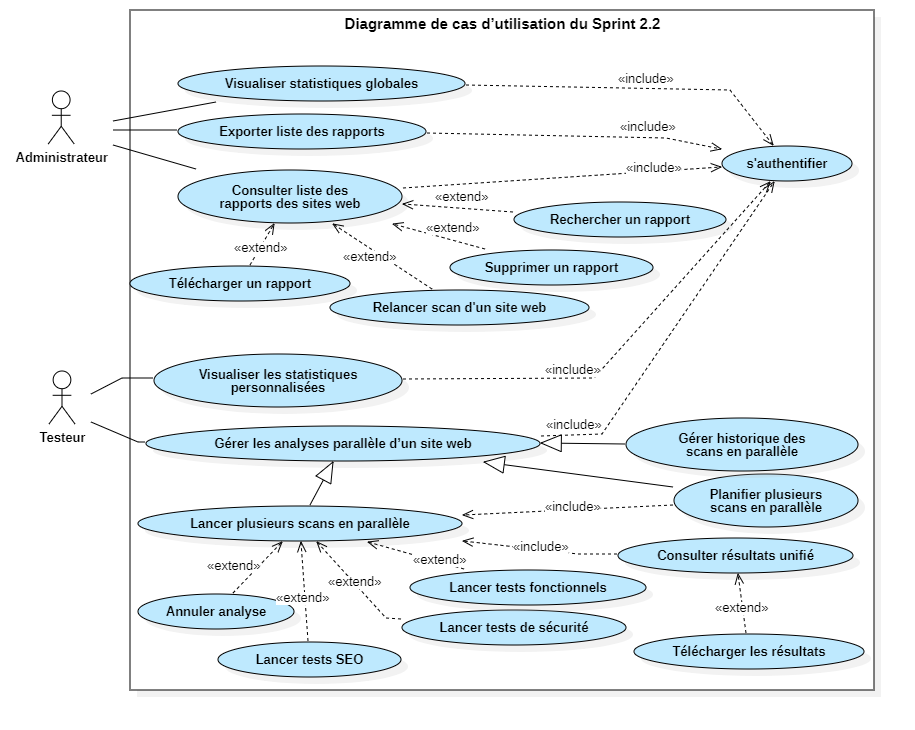
\includegraphics[width=\linewidth]{chapitres/ch4Sp2/section/sprint2.2/img/LastUseCaseSprint2.2.png}
    \caption{Diagramme de cas d'utilisation du sprint 2.2}
    \label{fig:caseS22}
\end{figure}
\vspace{-0.3cm}



\subsection{Conception du sprint 2.2}
Dans cette section, nous détaillons la conception des fonctionnalités développées au cours du sprint 2.2.

\subsection{Réalisation du sprint 2.2}
\begin{justify}
Dans cette section, nous présentons les principales interfaces développées durant cette sprint 2.2, en commençant par celles liées à l'exécution parallèle des tests, la gestion des rapports, puis la visualisation des statistiques.
\end{justify}
\begin{itemize}[label=$\bullet$]
    \item \textbf{Interface de la sélection des tests à exécuter} :  
    La figure \ref{fig:multiScanUI}\footnote{Voir annexe E : Figure \ref{fig:multiScanUI}} illustre l’interface permettant à l’utilisateur de sélectionner un ou plusieurs types d’analyses à effectuer (fonctionnelle, sécurité, SEO). Cette interface a été conçue pour offrir une interaction simple et efficace, favorisant l’exécution parallèle des différents scans.

    \item \textbf{Interface de visualisation consolidée des résultats} :  
    La figure \ref{fig:resultView}\footnote{Voir annexe E : Figure \ref{fig:resultView}} présente la vue unifiée des résultats d’analyse. Elle regroupe les vulnérabilités de sécurité, les erreurs fonctionnelles et les recommandations SEO dans une seule interface pour faciliter la lecture croisée et la prise de décision.

    \item \textbf{Interface de gestion des rapports d’analyse} :  
    Comme illustré dans la figure \ref{fig:reportManagementUI}, cette interface permet à l’administrateur de rechercher, supprimer, exporter les rapports. Les filtres intégrés (type, date, utilisateur) rendent la gestion des rapports plus fluide et performante.
    \begin{figure}
        \centering
        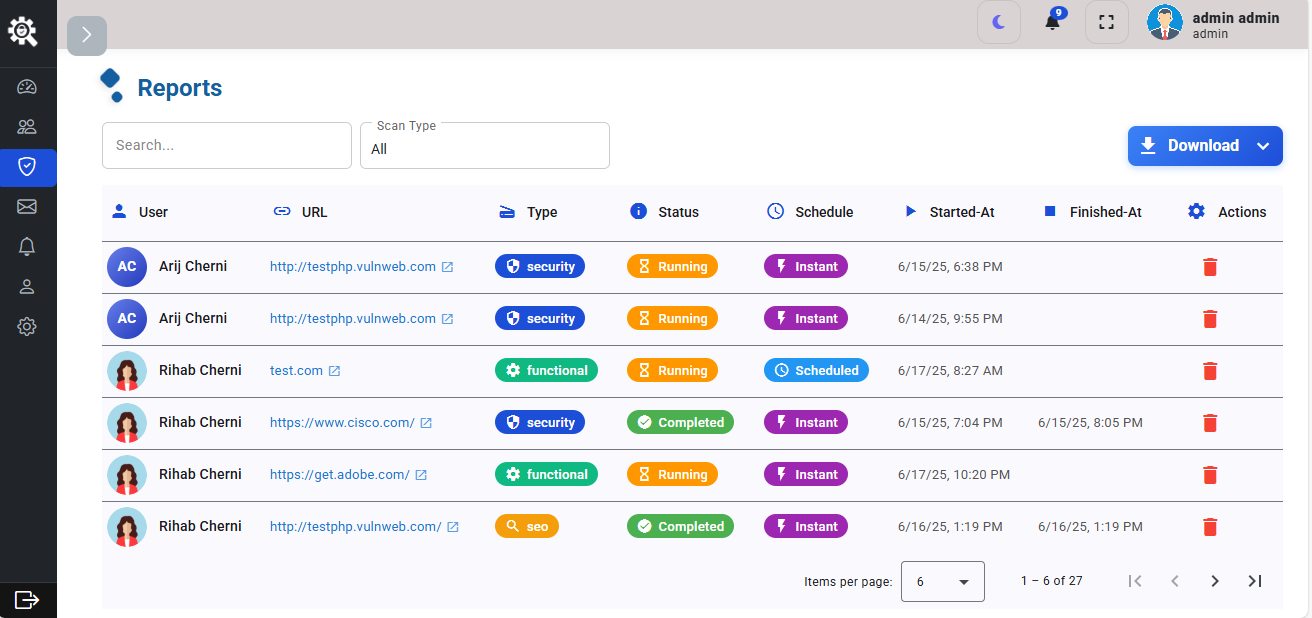
\includegraphics[width=\linewidth]{chapitres/ch4Sp2/section/sprint2.2/img/interface/reports-admin-liste.PNG}
        \caption{Caption}
        \label{fig:enter-label}
    \end{figure}

   \item \textbf{Tableau de bord utilisateur} :   La figure \ref{fig:testerdashboardUI}présente le tableau de bord dédié aux testeurs. Il affiche  des statistiques filtrables et interactives sur les campagnes de test, à travers des graphiques dynamiques.
    \begin{figure}[H]
        \centering
        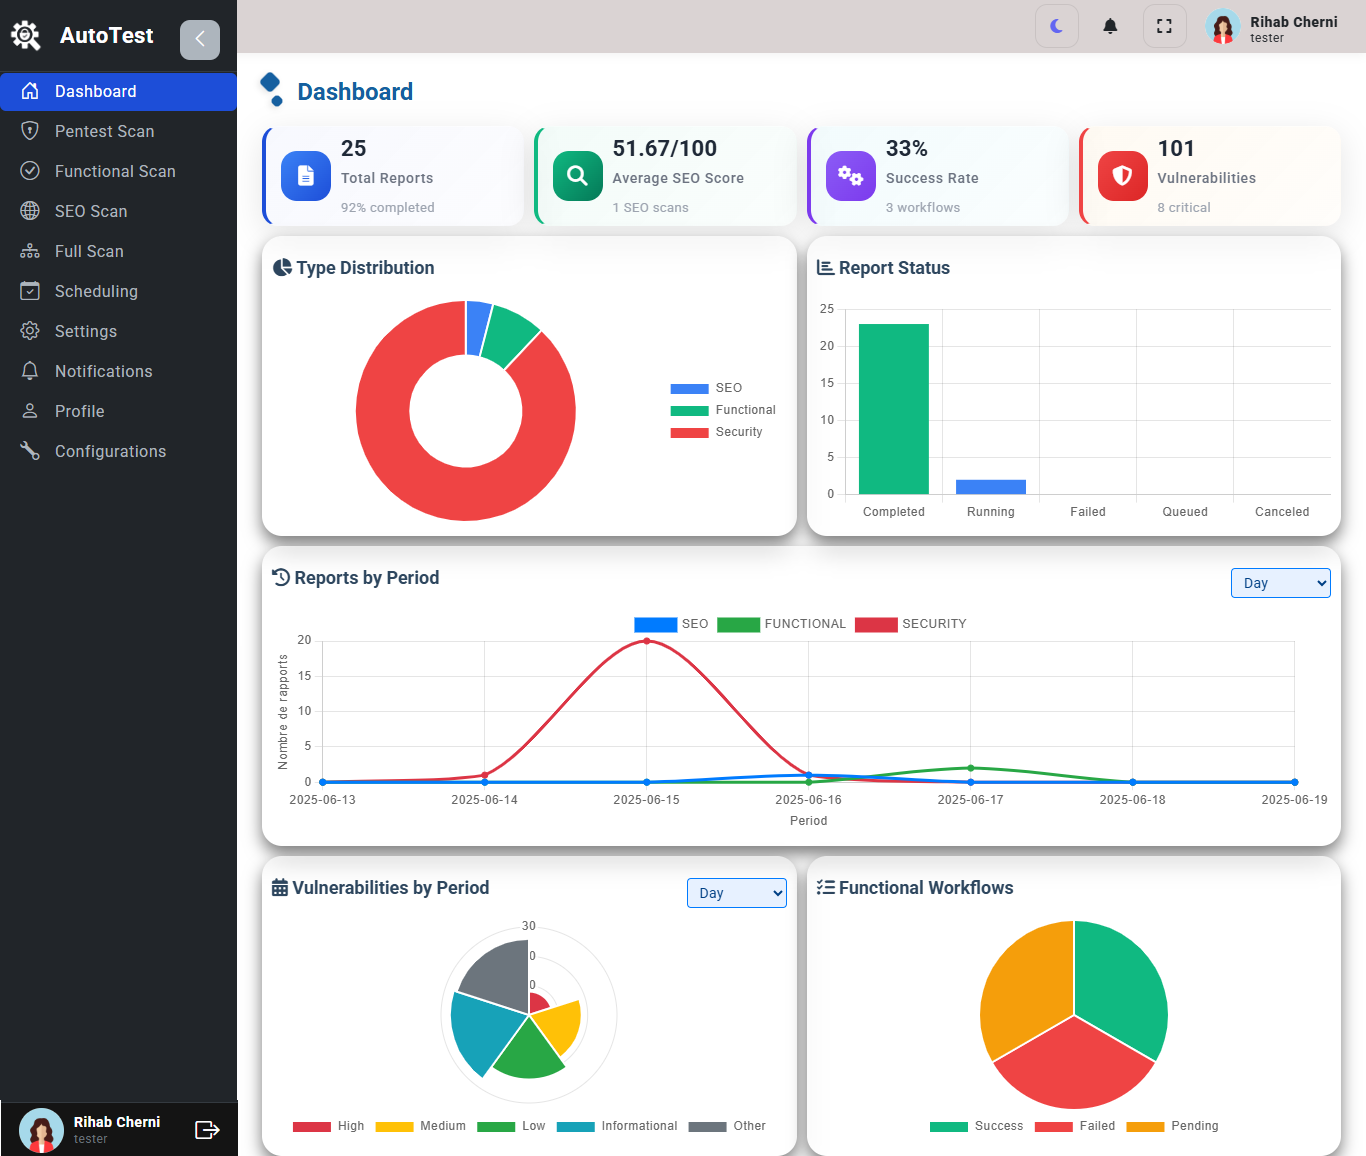
\includegraphics[width=\linewidth]{chapitres/ch4Sp2/section/sprint2.2/img/interface/tester-dashbaord.png}
        \caption{\centering Interface du tableau de bord testeur}
        \label{fig:testerdashboardUI}
    \end{figure}
    \vspace{-0.3cm}
    \item \textbf{Tableau de bord administrateur} :  
    Pour le profil administrateur, la figure \ref{fig:adminDashboardUI} met en évidence les indicateurs globaux sur l'activité de la plateforme : nombre de scans, utilisateurs actifs, types d’analyses effectuées, etc. Des filtres par période ou type d’analyse sont également disponibles.
    \begin{figure}[H]
        \centering
        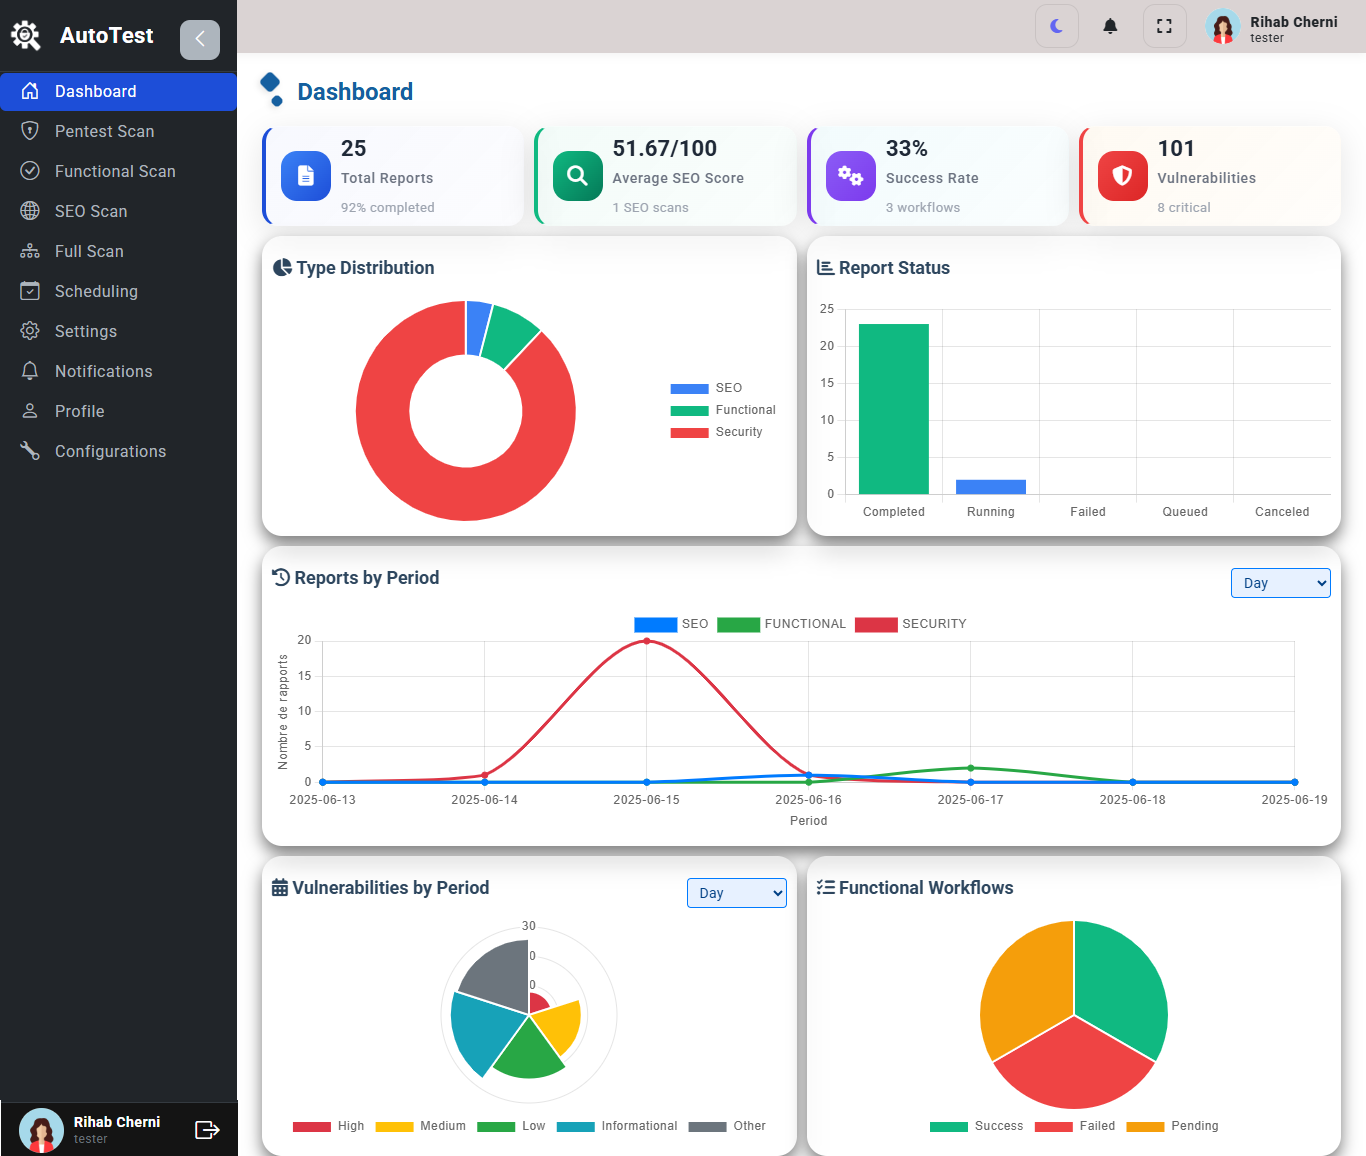
\includegraphics[width=\linewidth]{chapitres/ch4Sp2/section/sprint2.2/img/interface/tester-dashbaord.png}
        \caption{\centering Interface du tableau de bord testeur}
        \label{fig:testerdashboardUI}
    \end{figure}
    \vspace{-0.3cm}

    \item \textbf{Déploiement par conteneurisation} :  
    La figure \ref{fig:deploymentInterfaceUI}\footnote{Voir annexe E : Figure \ref{fig:deploymentInterfaceUI}} illustre le tableau de gestion du déploiement via Docker. Cette interface permet de visualiser le statut de chaque conteneur (backend, frontend, outils de scan), avec la possibilité de redémarrer individuellement les services.
\end{itemize}


    
    \section*{\texorpdfstring{Conclusion}{Conclusion}}
    \addcontentsline{toc}{chapter}{\textbf{Conclusion}}
    \begin{justify}
    Au terme de cette deuxième release, nous avons achevé la dernière phase de développement de notre application. Ce résultat a été atteint grâce à une démarche structurée, allant de l’analyse à la conception, puis à l’implémentation et à la réalisation finale.
\end{justify}

\end{justify}